\chapter{Graphen}

Ein Graph ist eine Struktur, die verwendet wird, um Beziehungen zwischen Objekten darzustellen.
Die Idee, Objekte durch Verbindungen zu verknüpfen, bildet die Grundlage für viele Anwendungen, unter anderem für die Routenplanung.
Graphen und (kürzeste) Pfade spielen auch darüber hinaus eine wichtige Rolle; in einem Wissensgraphen kann ein Pfad beispielsweise dafür stehen, dass eine Aussage wahr ist.
\autoref{graphs:fig:beispielgraph} zeigt einen Graphen, welcher im folgenden für Beispiele benutzt wird.

\begin{figure}[ht]
    \centering
    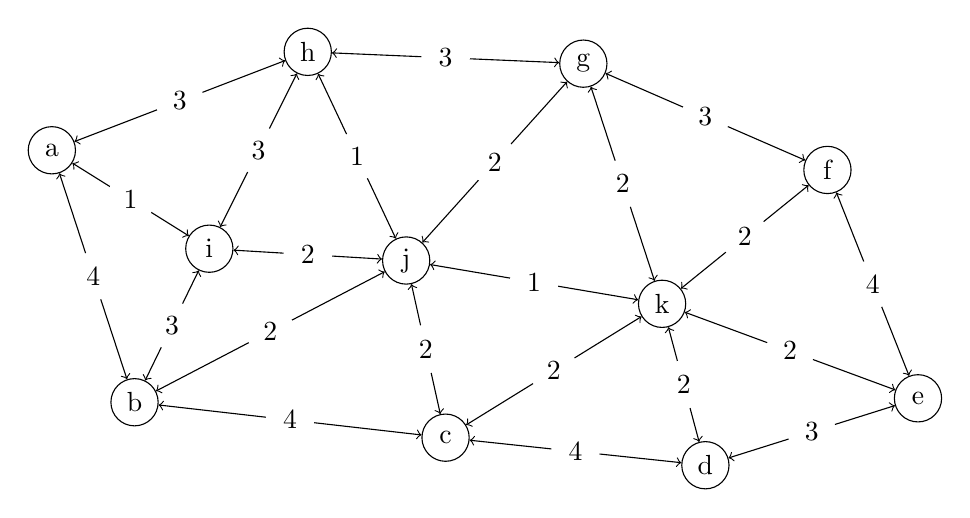
\begin{tikzpicture}
        % Nodes
        \node[circle, draw, minimum size=0.6cm, inner sep=0pt] at (0.5* 0.0, 0.5* 8.5)  (a)    {a};
        \node[circle, draw, minimum size=0.6cm, inner sep=0pt] at (0.5* 2.1, 0.5* 2.1)  (b)    {b};
        \node[circle, draw, minimum size=0.6cm, inner sep=0pt] at (0.5* 10.0, 0.5* 1.2)  (c)    {c};
        \node[circle, draw, minimum size=0.6cm, inner sep=0pt] at (0.5* 16.6, 0.5* 0.5)  (d)    {d};
        \node[circle, draw, minimum size=0.6cm, inner sep=0pt] at (0.5* 22.0, 0.5* 2.2)  (e)    {e};
        \node[circle, draw, minimum size=0.6cm, inner sep=0pt] at (0.5* 19.7, 0.5* 8.0)  (f)    {f};
        \node[circle, draw, minimum size=0.6cm, inner sep=0pt] at (0.5* 13.5, 0.5* 10.7)  (g)    {g};
        \node[circle, draw, minimum size=0.6cm, inner sep=0pt] at (0.5* 6.5, 0.5* 11.0)  (h)    {h};
        \node[circle, draw, minimum size=0.6cm, inner sep=0pt] at (0.5* 4.0, 0.5* 6.0)  (i)    {i};
        \node[circle, draw, minimum size=0.6cm, inner sep=0pt] at (0.5* 9.0, 0.5* 5.7)  (j)    {j};
        \node[circle, draw, minimum size=0.6cm, inner sep=0pt] at (0.5* 15.5, 0.5* 4.6)  (k)    {k};


        \draw[<->]  (a) edge node[circle, fill=white] {4} (b);
        \draw[<->]  (a) edge node[circle, fill=white] {3} (h);
        \draw[<->]  (a) edge node[circle, fill=white] {1} (i);

        \draw[<->]  (b) edge node[circle, fill=white] {4} (c);
        \draw[<->]  (b) edge node[circle, fill=white] {3} (i);
        \draw[<->]  (b) edge node[circle, fill=white] {2} (j);

        \draw[<->]  (c) edge node[circle, fill=white] {4} (d);
        \draw[<->]  (c) edge node[circle, fill=white] {2} (j);
        \draw[<->]  (c) edge node[circle, fill=white] {2} (k);

        \draw[<->]  (d) edge node[circle, fill=white] {3} (e);
        \draw[<->]  (d) edge node[circle, fill=white] {2} (k);

        \draw[<->]  (e) edge node[circle, fill=white] {4} (f);
        \draw[<->]  (e) edge node[circle, fill=white] {2} (k);

        \draw[<->]  (f) edge node[circle, fill=white] {3} (g);
        \draw[<->]  (f) edge node[circle, fill=white] {2} (k);

        \draw[<->]  (g) edge node[circle, fill=white] {3} (h);
        \draw[<->]  (g) edge node[circle, fill=white] {2} (j);
        \draw[<->]  (g) edge node[circle, fill=white] {2} (k);

        \draw[<->]  (h) edge node[circle, fill=white] {3} (i);
        \draw[<->]  (h) edge node[circle, fill=white] {1} (j);

        \draw[<->]  (i) edge node[circle, fill=white] {2} (j);

        \draw[<->]  (j) edge node[circle, fill=white] {1} (k);
    \end{tikzpicture}
    \caption{Beispielgraph}
    \label{graphs:fig:beispielgraph}
\end{figure}

\section{Definitionen}
Damit in den nachfolgenden Kapiteln sinnvoll argumentiert werden kann, ist es notwendig, einige Begriffe zu definieren.

\begin{definition}[Graph]
    Sofern nicht anders angegeben, wird im Folgenden Graph als Bezeichnung für einen endlichen, gerichteten Graphen mit Kantengewichten ohne Mehrfachkanten und Schleifen verwendet.

    Als Schreibweise wird $G = (V, E)$ verwendet, wobei $V$ die Knotenmenge und $E$ die Kantenmenge ist. Eine Kante ist ein Tupel $(t, h, w)$. $t \in V$ wird als \emph{Fuß} (Tail), $h \in V$ als \emph{Kopf} (Head) und $w \in \mathbb{R}^+$ als \emph{Gewicht} (Weight) bezeichnet. Gelegentlich wird auch nur $(t, h)$ geschrieben, um auszudrücken, dass zwei Knoten verbunden sind. Da ein Graph keine Mehrfachkanten zulässt, verweiste diese Schreibweise auch eindeutig das Kantengewicht.

    Wird $G$ als ungerichtet bezeichnet, dann gilt $(t, h, w) \in E \Leftrightarrow (h, t, w) \in E$ und $(t, h)$ kann als $\{ t, h \}$ geschrieben werden.
\end{definition}

Das Gewicht der Kanten ist hierbei auf positive reelle Zahlen begrenzt, da das Verwenden eines Kantengewichtes $0$ dazu führen kann, dass ein kürzester Pfad mehrfach einen Teilpfad der Länge 0 durchläuft.
Negative Kantengewichte erschweren die Definition und Argumentation, sodass hier auf diese nicht weiter eingegangen wird.

\begin{definition}[Nachbar]
    Sei $G = (V, E)$. Ein Knoten $u \in V$ heißt \emph{Vorgänger} eines Knoten $v \in V$ wenn $(u, v) \in E$. $v$ ist dann ein \emph{Nachfolger} von $u$.
    Ist $G$ ungerichtet, so spricht man beides mal von \emph{Nachbarn}.
\end{definition}

Die Anzahl der Nachbarn eines Knotens wird als sein \emph{Grad} bezeichnet, wobei bei gerichteten Graphen vom \emph{Eingangsgrad} und \emph{Ausgangsgrad} gesprochen wird.
Hat ein Knoten keine Vorgänger oder Nachfolger, so nennt man ihn \emph{isoliert}.

\begin{definition}[Pfad]
    Ein Pfad $p$ auf einem Graph $G = (V, E)$ ist eine Folge von Knoten $(v_1, \dotsc, v_n)$, für die gilt, dass benachbarte Knoten im Pfad durch eine Kante in $G$ verbunden sind.
    Der Knoten $v_1$ wird Startknoten, $v_n$ Zielknoten genannt.
    Die Summe der Kantengewichte aller Kanten $(v_i, v_{i + 1})$ wird \emph{Länge}, die Anzahl der Kantennutzungen ($n - 1$) \emph{Hop-Länge} genannt.
\end{definition}

Häufig wird für den Startknoten der Buchstabe $s$ (Source) und für den Zielknoten $t$ für Target verwendet.
Zwischen zwei Knoten kann es Pfade unterschiedliche Länge geben, dies führt zur Definition des kürzesten Pfades.

\begin{definition}[Kürzester Pfad]
    Ein Pfad $p$ ist \emph{ein kürzester Pfad}, wenn die Länge von $p$ unter allen Pfaden von $v_1$ nach $v_n$ minimal ist.
    Die Länge des kürzesten Pfades wird als \emph{Abstand} von $v_1$ und $v_n$ bezeichnet.

    Die Funktion ${spd} \colon V \times V \to \mathbb{R}^+ \cup \{ \infty \} $ (shortest path distance) weist einem Knotenpaar den Abstand zu, wobei dieser unendlich ist, wenn kein Pfad zwischen ihnen existiert.
    Sei dann $P \subset V \times V$ die Menge der Knoten, zwischen denen ein Pfad existiert.
    Dann weist ${sp} \colon P \to V \times V \times \dots \times V$ (shortest path) einem Knotenpaar einen kürzesten Pfad zu.
\end{definition}

Zusätzlich zum Finden eines Pfades zwischen zwei Knoten ist es häufig notwendig die kürzesten Pfade von einem Knoten zu allen anderen Knoten zu finden.
Auch die Umkehrung dieses Problem ist Interessent, also die kürzesten Pfade von allen Knoten zu einem Knoten zu bestimmen.
Diese Probleme sind äquivalent, da das Finden aller kürzesten Pfade zu einem Knoten auf einem Graph $G$ dem Finden aller kürzester Pfade auf dem Umkehrgraph $G^T$ entspricht.

\begin{definition}[Transponierter Graph]
    Sei $G = (V, E)$ ein Graph. Dann ist $G^T = (V, E^T)$ mit $(t, h, w) \in E \Leftrightarrow (h, t, w) \in E^T$ der \emph{transponierte Graph} von $G$.
\end{definition}

Ein ungerichteter Graph ist hier bei selbst ein transponierter Graph.

\begin{definition}[Hitting-Set]
    Sei $G = (V, E)$ ein Graph und $P$ eine Menge an Pfaden auf $G$.
    Ein Hitting-Set $H \subset V$ ist eine Menge an Knoten, so dass jeder Pfad $p \in P$ mindestens einen Knoten aus $H$ enthält
\end{definition}

Ein triviales Beispiel für ein Hitting-Set ist $V$ selbst, im Weiteren sind jedoch möglichst kleine Hitting-Sets nützlich.
Das Finden kleinst möglicher Hitting-Sets ist NP-vollständig \cite{Kar72}.
Der Greedy-Algorithmus \ref{graphs:alg:greedy-hitting-set} bietet jedoch eine Approximation in polynomieller Zeit an.

\begin{algorithm}
    \caption{Greedy Hitting-Set}
    \begin{algorithmic}[1]
        \Require Knotenmenge $V$, Pfade $P$ über $V$
        \Ensure Hitting-Set $H$

        \State $H \gets \emptyset$

        \State

        \While{$P \neq \emptyset$}
        \State Wähle $v \in V$ mit $\abs{ \{ p \mid p \in P \colon v \in p \}}$ maximal
        \State $H \gets H \cup \{  v \}$
        \State $P \gets P \setminus \{p \in P \mid v \in p\}$
        \EndWhile

        \State

        \State \Return $H$
    \end{algorithmic}
    \label{graphs:alg:greedy-hitting-set}
\end{algorithm}


\section{Graphentypen}
\subsection{Straßengraphen}\label{graphs:strassengraphen}

Straßengraphen stellen eine spezielle Klasse von Graphen dar, die  Eigenschaften aufweisen, welche sie von allgemeinen Graphen abgrenzen.
Eine ihrer auffälligsten Merkmale ist, dass sie nahezu planar sind, sie also fast in der Ebene darstellen lassen, wobei Ausnahmen in Form von Über- und Unterführungen existieren.
Die Kantengewichte können etwa dem Luftlinienabstand oder der Reisezeit entsprechen, wobei sich letzter im Verlauf der Zeit ändern, etwa durch Stau oder Bauarbeiten.
Sie haben einen relativ geringen durchschnittlichen Knotengrad, Kreuzungen von mehr als zwei Straßen sind selten.

Sie besitzen sie eine hierarchische Struktur: Einfach gesagt, je schneller auf einer Straße gefahren werden darf, desto wichtiger is diese für das Finden von kürzesten Pfaden.
Die Wichtigkeit der benutzten Straßen eines kürzesten Pfades steigt im Allgemeinen an, bis etwa eine Autobahn erreicht wird, und nimmt schließlich wieder ab, bis das Ziel erreicht wird.

Eine weitere Eigenschaft dieser hierarchischen Struktur ist, dass hinreichend lange Pfade durch ein vergleichbar kleines Hitting Set getroffen werden.
Diese Knoten können etwa Autobahnkreuzen und Anschlussstellen sein.
Diese Beobachtung führt zur Definition der sogenannten Highway Dimension, einem Konzept, das von \cite{abraham2010highway} eingeführt wurde.

\subsection{Nicht-Straßen-Graphen}

Alle Graphen, die keine Straßengraphen sind, werden als Nicht-Straßen-Graph bezeichnet.
Da sie durch den Ausschluss der Straßengraphen definiert werden, haben sie keine gemeinsamen Eigenschaften, jedoch könne weite Teilklassen definiert werden.

\subsubsection{Sichtbarkeitsgraphen}

\todo{Funke. Was soll ich schreiben Stichwörter pls, Gummiband Eigenschaft}

\begin{definition}[Sichtbarkeitsgraph]
    Sei $V$ eine Menge an Punkten in einem euklidische Raum $A$. Sei $P$ eine Menge an Polygonen im selben Raum.

    Der Sichtbarkeitsgraph $G = (V, E)$ enthält alle Kanten $(t, h)$, die kein Polygon schneiden.
    Ihr Kantengewicht ist durch den euklidischen Abstand defniert.
\end{definition}



\subsubsection{Die Graphen im Detail}

\todo{Bilder}

\section{Dijkstra Algorithmus}

Die Angabe wie aufwändig die Suche eines kürzesten $(s, t)$ Pfades für einen Computer ist, lässt sich schwer in einer Metrik ausdrücken, denn die Zeit, welche für die Suche benötigt wird, ist von der verwendeten Hardware abhängig.
Ein Möglichkeit diese Aufwändigkeit zu beziffern, ist der \emph{Dijkstra Rank}.
Dieser gibt an, wieviele Knoten in einer Dijsktra-Suche von $s$ aus expandiert werden müssen, bis man von $t$ erreicht.

\todo{Ich habe gelesen, dass Dijkstra die meiste Zeit in Queue verbringt. Kann ich das wieder finden, oder selber perfen?}

Ebenfalls interesannt sind die Warteschlagen (Queue) Operationen, diese können auch Hinweise darauf geben, was genau die Suche in einem Graph so teuer macht.
Hierbei sind die \emph{Queue Pops} die Anzahl, wie oft Knoten aus der Warteschlange entommen wurde.
Wenn eine Warteschlange mit \emph{Decrease-Key} Funktion benutzt wird, unterscheidet sie sich nicht vom Dijsktra Rank.
Die \emph{Queue Pushs} geben an, wie oft Knoten aus der Warteschlange entommen werden.


\todo{Dijkstra Algorithmus erklären und Dijkstra Paper zitieren}
\begin{algorithm}[ht]
    \caption{Dijkstra Algorithmus}
    \begin{algorithmic}[1]
        \Require Graph $G = (V, E)$, Startknoten $s \in V$, Zielknoten $t \in V$
        \Ensure ${dist}$, ${pre}$
        \State // Initialisiere Distanz- und Vorgänger-Funktion
        \ForAll{$v \in V$}
        \State ${dist}(v) \leftarrow \infty$
        \State ${pre}(v) \leftarrow {none}$
        \EndFor


        \State
        \State // Initialisiere Vorrangwarteschlange
        \State ${dist}(s) \leftarrow 0$
        \State $Q\leftarrow \{ s \}$

        \State
        \While{$Q \neq \emptyset$}
        \State $u \leftarrow{extract\_min}(Q)$\label{graphs:dijkstra:pop}

        \State
        \State // Beende frühzeitig wenn Zielknoten gefunden wurde
        \If {$u = t$}
        \State \textbf{break}
        \EndIf

        \State
        \State // Aktualisiere Nachbarn
        \ForAll{$(u, v, w) \in E$}
        \If {${dist}(u) + w < {dist}(v)$}
        \State ${dist}(v) \leftarrow {dist}(u) + w$
        \State ${pre}(u) \leftarrow v$
        \State $Q = Q \cup \{ v \}$
        \EndIf
        \EndFor

        \EndWhile

        \State
        \State \Return ${dist}$, ${pre}$
    \end{algorithmic}
\end{algorithm}


\section{Dateiformat}

Die in dieser Arbeit verwendeten Graphen sind im \emph{.fmi} Dateiformat gespeichert, welches wie folgt definiert ist:

\begin{definition}[FMI Dateiformat]
    Eine Datei im .fmi Format besteht aus den folgenden Zeilen (in der angegebenen Reihenfolge):
    \begin{enumerate}
        \item
              Beliebig viele Kommentarzeilen, die mit einem \# beginnen.

        \item
              Eine leere Zeile.

        \item
              Eine Zeile, die die Anzahl der Knoten enthält.

        \item
              Eine Zeile, die die Anzahl der Kanten enthält.

        \item
              Knoten-Zeilen im Format: \texttt{KnotenId1 KnotenId2 Breitengrad Längengrad Höhe}

        \item
              Kanten-Zeilen im Format: \texttt{FußId1 KopfId2 Gewicht Typ Geschwindigkeit}

    \end{enumerate}
\end{definition}

Für die in dieser Arbeit verwendeten Graphen sind die Felder für Höhe, Typ und Geschwindigkeit nicht von Bedeutung, sie enthalten jeweils den Wert 0.

\section{Datenstrukturen}

Die Wahl der Datenstruktur, welche ein

Vertices sind natürliche Zahlen bzw uint32.
Ein Graph enthält idealerweise keine isolierten Knoten.
isolierte Knoten sind doof für dijkstra und co.
Die Menge der Knoten ist definiert durch Ihre Anzahl.
Gibt es $n \in \mathbb{N}$ Knoten, so sind es $0, \dotsc, n - 1$.
Ein Graph der diese Eigenschaft nicht erfüllt, kann durch eine Mapping der Knoten in die Form gebracht werden.

Jenachdem was mit dem Graph gemacht werden soll, sind verschiedene Eigenschaften von Vorteil.
Manchmal ist eine effiziente Nachbar Abfrage wichtig,
Manchmal das bearbeiten des Graphes, einfügen oder löschen von Knoten

Es wurde ein dyn Trait benutzt, welches eine Overhead hat und kein inlining zulässt.
Dafür lassen sich verschiedene Methoden vergleichen.

Die Grundlegenden Implementierungen kennen nur ihre Vorgänger.
Ein Reversibe Graph besteht aus einem Graph und seinem Umkehrgraph.
Gleiche Datenstruktur.

\subsection{VecVecGraph}
Ein Vec mit pro Knoten ein Vec.
Der innere Vec speichert Tuple aus (Vertex, Distanz).
Der innere Vec ist nach Vertex sortiert.

Ein Knoten kann so mit eine binären Suche gefunden werden.
Doch ab einem großen Grad wird diese Suche teuer.
Das einfügen und Löschen ist auch etwas teuere, da die übrigen Elemente geschoben werden müssen

Das finden von Nachbarn geht aber schnell, weil kein unbenutzer Platz dazwischen ist.

\subsection{VecHashMap}
Ein Vec mit pro Knoten eine HashMap
Die innere HashMap speichert Vertex -> Distanz.
So kann schnell ein Knoten gefunden werden.

Das finden von Nachbarn ist etwas langsamer, da unbenutzter Platz zwischen den Hash Einträgen.

Das einfügen und löschen ist günstig.

Vielleicht wäre IndexMap noch spannend.
Schnelles finden von Nachbarn.
Schnelles Iterieren.

Einfügen und löschen etwas teuerer.

\subsection{VecGraph}
Zwei Vecs.
Ein Index Vec mit pro Knoten ein Eintrag (u32, u32).
Dieser Eintrag gibt den Startindex und Stopindex des des zweiten Vecs an.
Dieser ist ein Vec (Vertex, Distanz).

Das bietet den Vorteil, dass man die Kanten zusätzlich sortieren kann, für besser Cache lokalität.
Kanten häufig benutzter Knoten können so an einem Ende des Vec grupiert werden.